\section{Introduction}
    
    As the size and complexity of engineering systems grows the time and expense for setting up 
    analysis models grows with them. Multidisciplinary Design Analysis and Optimization (MDAO)
    frameworks such as OpenMDAO\cite{Gray2012} and ModelCenter have enabled a new level of analysis tool integration 
    and paved the way for models of with more analysis tools and increasing numbers of multidisciplinary couplings. 
    Such complex models present a distinct challenge proper implementation of any given solution strategy . 
    
    We propose the use of graph based problem formulation that generally describes a
    given problem, supports algorithmic manipulation to find beneficial solutions strategies, and enables automated 
    implementation of those strategies inside an MDAO framework. In order to serve that purpose, the graph includes the following information: 
    \begin{itemize}
       \item Discipline Analyses 
       \item Discipline State Variables and Residuals
       \item Design Variables
       \item Constraints
       \item Objective or Objectives
       \item Coupling Constraints
       \item Parameters
    \end{itemize}
    Notably absent from the preceding list are any kind of solvers, optimizers, or other iterative solution finding tools. 
    At it most basic, a problem formulation includes only information about what is being sought after in a given problem, or what the
    goals of a given problem are. It need not contain any information about solution paths or strategies to reach those goals. 

    We define a problem specification striped down to it's most essential parts to be the 
    Fundamental Problem Formulation (FPF). By definition, the FPF for any given problem will be constant regardless 
    of which MDAO framework, optimization architecture, optimization algorithm, or iterative solver is used to solve the problem.

    The graph based syntax used in this work is based on the Design Structure Matrix (DSM). 
    This provides several key features that make it useful for working with large scale MDAO problems. 
    It provides a rigid structure that can be easily manipulated with a wide range of well establish graph-theory algorithms 
    for the purposes of problem decomposition. It also provides a means for testing a given 
    problem formulation to check if it is the FPF, and if not to reduce it to the FPF. Lastly, it lends itself 
    well to interacting with MDAO frameworks. 

\section{Specific vs Fundamental Problem Formulation }
    For a simple, notional problem  is given as follows: 

    \begin{align}
        given & \ \ A: {x,y} \rightarrow {m,z} \notag
        \\      & \ \ B: {x,z} \rightarrow {y^t} \notag
        \\min. &\ \ f(m) \notag
        \\w.r.t. & \ \ x,y,z \notag
        \\s.t. & \ \ g(y^t,y) = 0
        \label{eqn:simple}
    \end{align}

    Where $A$ and $B$ represent analysis tools, $f,g$ are the objective and constraint functions respectively. 
    Equation \ref{eqn:simple} makes an inherent assumption about the solution strategy for the problem. 
    Analysis $A$ outputs $z$ which is an input to $B$. Hence, $A$ should be run before $B$ with 
    the $y$ being iterated on to convergence with $y^t$. However, a different solution could be equally valid and still represent
    the same fundamental problem: 

    \begin{align}
        given & \ \ B: {x,z} \rightarrow {y} \notag
        \\      & \ \ A: {x,y} \rightarrow {m,z^t} \notag
        \\min. &\ \ f(m) \notag
        \\w.r.t. & \ \ x,y,z \notag
        \\s.t. & \ \ g(z^t,z) = 0
        \label{eqn:simple2}
    \end{align}

    Equation \ref{eqn:simple2} differs only slightly from Eqn. \ref{eqn:simple}. $A$ is now dependent on the output of $B$, 
    and $z$ will be iterated on to satisfy $g$. Now the problem can be solved by running $B$ first and then $A$.
    Since the formulations in Eqn. \ref{eqn:simple} and \ref{eqn:simple2} both describe the same problem and neither can be the FPF. 
    There must be a more fundamental description of the problem that is common between them. We present the FPF as follows: 

    \begin{align}
        given & \ \ A: {x,y} \rightarrow {m,z^t} \notag
        \\      & \ \ B: {x,z} \rightarrow {y^t} \notag
        \\min. &\ \ f(m) \notag
        \\w.r.t. & \ \ x,y,z \notag
        \\s.t. & \ \ g1(z^t,z) = 0 \notag
        \\     & \ \ g2(y^t,y) = 0
        \label{eqn:simple_fpf}
    \end{align}

    The FPF in Eqn. \ref{eqn:simple_fpf} differs from both Eqn. \ref{eqn:simple} and Eqn. \ref{eqn:simple2} because it has 
    two constraints which both must be met. The presence of both of these constraints fully decouples the problem so that 
    either $A$ or $B$ could be run first or both could be run simultaneously. By removing either constraint, and replacing 
    it with a direct dependence between the two analyses you could regain the earlier two problem formulations.     


\section{Using DSM for Problem Formulation}

    As shown above, the mathematical language for specifying problem formulations is very general and can be used both for 
    fundamental and specific problem formulations. Tedford and Martins used the above mathematical syntax to specify the 
    FPF for a set of test problems and also to describe specific formulations for solving them with a 
    number of optimization architectures\cite{Tedford2009}. Their work demonstrates clearly how multiple specific 
    problem formulations can all relate back to a common FPF. 
    
    The challenge with using this traditional mathematical syntax is that it is not easily manipulated or analyzed. 
    A number of matrix based methods have been used successfully to translate the mathematical syntax into a more useful computational form. 
    Steward's Design Structure Matrix (DSM) is a square adjacency matrix which captures the relationship between analysis tools where off 
    diagonal elements of the matrix indicate coupling\cite{Steward1981}. Since a DSM describes a square adjacency matrix, 
    it can be represented in an equivalent directed graph where nodes represent analysis tools and 
    edges represent information dependence between those tools. The ordering of elements in a DSM can be used to indicate 
    execution order.  For more complex problems, choosing the proper order to run analysis tools is a non-trival task. 
    Rogers et. al developed DeMAID to manipulate a DSM to find an ordering for analysis tools that 
    reduces the cost of solving highly coupled systems\cite{Rogers1996}. This re-ordering yields multiple specific problem 
    formulations which all solve the same FPF. In other words, manipulation of the DSM does not fundamentally alter
    the problem formulation, which makes DSM an excellent foundation for specifying the FPF itself. Traditional DSM only captures information 
    about data dependency between analyses. Objective and constraint information is missing from the description of the problem. 
    
    An alternate matrix based syntax, called a Functional Dependency Table (FDT), was proposed by Michelena and Papalambros. 
    FDT represents the relationship between functions, including objectives and constraints, and specific variables that affect 
    them\cite{Michelena1997}. Similar to DSM, FDT also describes an adjacency matrix of a graph. Unlike the DSM graph, 
    however, the graph is undirected and nodes can represent analysis tools, objectives, 
    or constraints. Edges between nodes represent a dependence on the same 
    variable. Wagner and Papalambros made use of the FDT to solve a graph partitioning problem that yielded 
    more efficient optimization problem decompositions\cite{Wagner1993}. While FDT succeeds at capturing the 
    information about objectives and constraints, it neglects the data dependency captured by DSM. For instance, 
    although we know from the FPF in Eqn. \ref{eqn:simple_fpf} that the objective, $f$, is dependent on the 
    output of analysis $A$, you could not determine that from the FDT in Fig. \ref{fig:FDT_simple} alone. 
    
    [TODO: There is more recent research to cite here. e.g. Allison's Work.]

    \begin{figure}
        \begin{center}
        \begin{tabular}{|c|c|c|c|c|c|c|}
            \hline
                 & $x$ & $y$ & $y^t$ & $z$ & $z^t$ & m \\ \hline
            $A$  & 1  & 1    &       &     &       &   \\ \hline
            $B$  & 1  &      &       & 1   &       &   \\ \hline
            $f$  &    &      &       &     &       & 1 \\ \hline
            $g1$ &    &      &       & 1   & 1     &   \\ \hline
            $g2$ &    & 1    & 1     &     &       &   \\
            \hline
        \end{tabular}
        \caption{Functional Dependency Table (FDT) for Eqn. \ref{eqn:simple_fpf} \label{fig:FDT_simple}}
        \end{center}
    \end{figure}

    Lamb and Martins included the variables, objectives, and constraint functions as nodes in an Extended 
    DSM (XDSM) in order to capture a more complete description of solution strategies for MDAO problems\cite{Lambe2012}. By adding in those 
    elements, they partially combined a traditional DSM with an FDT. This allows XDSM to represent data 
    dependency between multiple analysis tools as well as between analysis tools and objective/constraint functions. 
    With the additional information included in an XDSM Lu and Martins applied both ordering and partitioning 
    algorithms on an MDAO test problem named the Scalable Problem \cite{Lu2012}. 

    \begin{figure}
        \begin{center}
        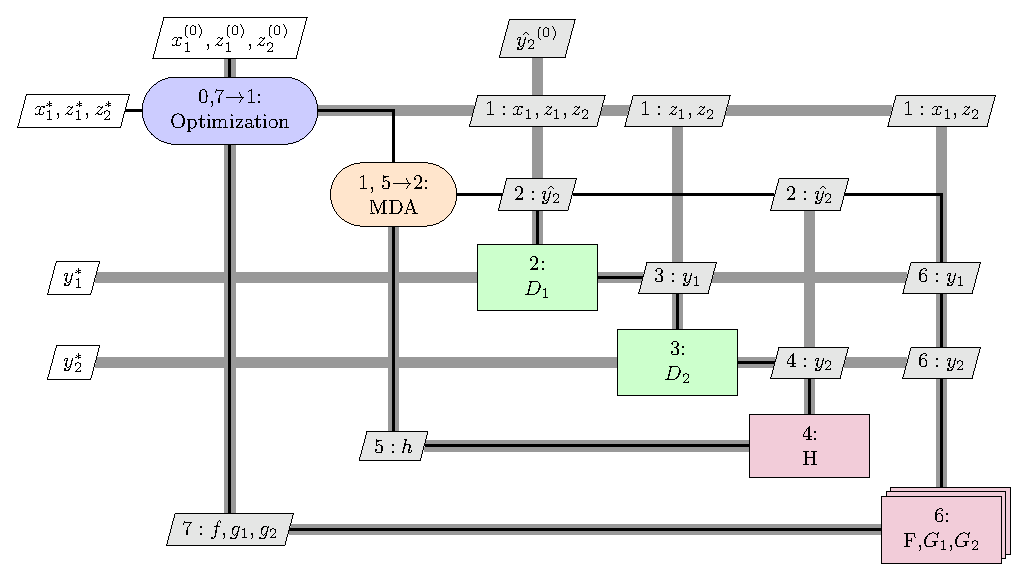
\includegraphics[height=.25\textheight]{XDSM/simple}
        \caption{XDSM for Eqn. \ref{eqn:simple}, with a gauss-siedel iteration and MDF solution architecture. \label{fig:XDSM_simple}}
        \end{center}
    \end{figure}

    Although XDSM captures part functional aspects of FDT, it  leaves out the variables themselves. As a result, all variable information is aggregated 
    so that for the problem from Eqn. \ref{eqn:simple_fpf} you can say that $A$ depends on $B$ or vice versa, but you can't identify which 
    individual variables are interacting in the dependency cycle. Without the detailed variable information, you can't construct the compatibility 
    constraints necessary to implement the problem. Additionally, XDSM requires the use of solver and optimizer blocks to represent 
    the relationship between design variables and objectives/constraints. By introducing solver or optimizer blocks XDSM automatically provides
    some kind of solution strategy. The XDSM for Eqn. \ref{eqn:simple} is given in Figure \ref{fig:XDSM_simple}. 
    This diagram is shown with an assumed gauss-siedel iteration scheme and a MDF solution architecture. 
    Hence XDSM is too specific for use with a fundamental problem formulation. 

    By taking XDSM, removing the solver/optimizer nodes and adding in nodes for each variable we are able to fully describe 
    the problem formulation for a general MDAO problem. In the following sections we describe the necessary syntax for specifying a 
    problem formulation withing a DSM and show how to make use of the resulting graph to find the FPF from any given graph. For completeness we 
    also present algorithms for converting between the general DSM and the more specific formulations discussed above. 


